% PAGINA INICIAL DO PRIMEIRO ARTIGO
\mytitle{A História do Universo: Era Primordial} % Título do Artigo    
\addchaptersummary{A História do Universo: Era Primordial}{Sumario/Figs_Sumario/FigArtigo1.jpg}{Neste texto aprenderemos sobre a origem dos átomos e também sobre a luz mais antiga do universo: a radiação cósmica de fundo, de 13,8 bilhões de anos.}{Luiz Felipe Demétrio} 
% Comando para adicionar o título do artigo (deve sempre ficar após o comando \mytitle) no sumário bem como uma figura, resumo e autor(a) do mesmo (obs: o diretório da figura deve ser especificado na segunda variável como mostra esse exemplo. Recomenda-se o uso de figuras quadradas.)
\newcommand{\artigoum}{\begin{center}\textcolor{base}{\MakeUppercase{A História do Universo: Era Primordial}}\end{center}} % Comando para adicionar o nome do artigo nas referências. Altere \artigoum para \artigodois, \artigotres de acordo com o total de artigos da edição e adicione o mesmo comando antes da sua seção no arquivo Referencias.tex

% Use o ambiente multicols para textos em duas colunas.
\begin{multicols}{2} % Tudo o que estiver dentro desse ambiente ficará no layout de duas colunas. 
% Pule uma linha entre \begin{multicols} e o texto
Bem-vindo a mais um texto sobre a História do Universo. Vimos no \href{https://drive.google.com/file/d/1D3q3ixp0qqPirSmoWL_jqtcO3WCsY0qJ/view}{último texto} que a fusão estelar não explica a origem dos elementos químicos leves, como hidrogênio e hélio. Mas, na verdade, eu enganei vocês: o buraco é bem mais embaixo. Veja bem, todos os elementos químicos são feitos de átomos. Mas de onde vem os átomos? Continue lendo e você descobrirá .

\mysubtitle{Rebobinando o filme do Universo} % Subtítulo do Artigo  
%

Como já vimos, o universo expande, e isso nos fornece muita informação sobre seu comportamento. Isso significa que, se ``rebobinarmos o filme'' do universo, então, no passado, ele deveria ter sido ``menor''\footnote{Lembrando que o universo é \textbf{infinito}, mas as \textbf{distâncias} dentro dele variam com o tempo.}, e, consequentemente, mais quente e denso\footnote{É isso que chamamos de \textit{Big Bang}: a ideia de que o universo evoluiu de um estado quente e denso para o que vemos hoje, capaz até de gerar vida.}.

% Para aspas duplas de abertura, use dois caracteres de acento grave (ou crase. Para aspas duplas de fechamento, use dois caracteres de aspas simples. Ex: ``palavra ou frase''. Use o comando \footnote{} para notas de rodapé.

Como as escalas de distância do universo primordial eram menores, isso se aplica também para os comprimentos de onda $\lambda$ da luz. A energia $E$ da luz em função de seu comprimento de onda é dada pela relação de Planck

\begin{equation}\label{Eq1}
    E = \frac{hc}{\lambda}\, ,
\end{equation}

\noindent em que $h$ é a constante de Planck e $c$ a velocidade da luz. Vemos então que energia e comprimento de onda são inversamente proporcionais: quanto menor o comprimento de onda, maior a energia. 

% Use o comando \noindent para tirar a indentação de um parágrafo e o comando \ref{} para citar a equação no texto de acordo com o seu rótulo no comando \label{Eq1}. 

Sabemos também que, no passado, o comprimento de onda da luz era menor, ou seja, ela possuía muito mais energia do que tem hoje em dia. Em particular, nas eras primordiais do universo, ela tinha energia suficiente para destruir átomos.

Uma forma de entender isso é imaginar um grupo de amigos abraçados em uma praia, como os da Figura \ref{fig:amigos}. Imagine agora que uma onda passa pelo nosso grupo de amigos, uma onda bem fraquinha. Como ela é fraca, ela irá apenas incomodar os amigos um pouco, mas não irá desfazer o abraço coletivo.

\begin{figure}[H]
	\centering
	
\includegraphics[width=\linewidth]{Figuras/Artigo1/Beach.png}
	\caption{Amigos de mãos dadas. Feito pelo autor no \href{https://www.canva.com/}{Canva}.}
	\label{fig:amigos}
\end{figure}

Porém, se a energia da onda aumentar, ela poderá vir a desfazer a roda, a não ser que os amigos façam mais força para se segurarem. Obviamente, se a onda for muito muito forte, eles jamais conseguirão manter o abraço coletivo.

Agora que entendemos nossa experiência imaginária na praia, voltemos para o universo primordial. A situação é totalmente análoga: os prótons e elétrons são muito amigos, e sentem uma atração (elétrica) muito forte, querendo ficar abraçados. O nome desses abraços coletivos são \textit{átomos} (Figura \ref{fig:bohr}). Na analogia, a onda faz o papel da luz.

\begin{figure}[H]
	\centering
	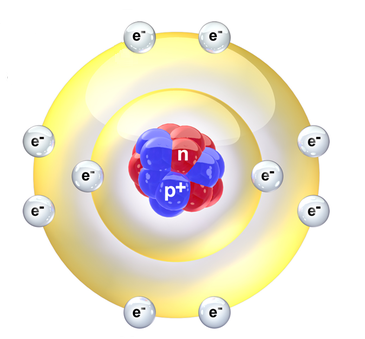
\includegraphics[width=0.9\linewidth]{Figuras/Artigo1/Bohr.png}
	\caption{Um átomo é composto por elétrons de cargas negativa, com um nucleon de prótons com carga positiva e nêutrons sem carga. Fonte: \href{https://en.wikipedia.org/wiki/File:Blausen_0342_ElectronEnergyLevels.png}{Wikipédia}.}
	\label{fig:bohr}
\end{figure}

\mysubtitle{Nucleossíntese primordial}

O universo primordial era então como uma praia cheia de ondas muito poderosas, que destruíam os átomos. Porém, conforme ele se expandiu, chegou a um ponto no qual as ondas foram perdendo energia, até que elas permitissem a formação de núcleos de átomos. Esse instante é muito importante para a História do Universo, sendo chamado de \textbf{Nucleossíntese Primordial}, e ocorreu cerca de 10 a 20 minutos depois do que chamamos de ``origem'' do universo.
	
Em seguida, ocorreu a chamada \textbf{Recombinação}, quando os núcleos capturaram elétrons e foram formados os primeiros átomos de hidrogênio, hélio, e outros elementos leves. Isso  ocorreu há cerca de 13,8 bilhões de anos, aproximadamente 380 mil anos depois da Nucleossíntese Primordial. Em seguida, conforme o universo evoluiu, eles se condensaram em elementos mais pesados, depois estrelas e galáxias.

A origem dos átomos por si só já é uma consequência incrível do modelo do Big Bang, pois a abundância de hidrogênio e hélio em nosso universo não é explicada por outros modelos cosmológicos.  Porém, surge uma outra pergunta: agora que a luz primordial perdeu energia e parou de colidir com os átomos e destruí-los, o que aconteceu com ela?

\mysubtitle{Radiação Cósmica de Fundo(CMB)}

Desde o momento da recombinação, os fótons\footnote{Partículas de luz.}  não conseguiram mais destruir os átomos, passando a vagar livremente pelo universo. Eles então vagaram e vagaram, por todo o cosmos, ou melhor, até a parte do cosmos que tiveram tempo de andar\footnote{Porque a velocidade da luz é finita.}. 

\begin{figure}[H]
	\centering
	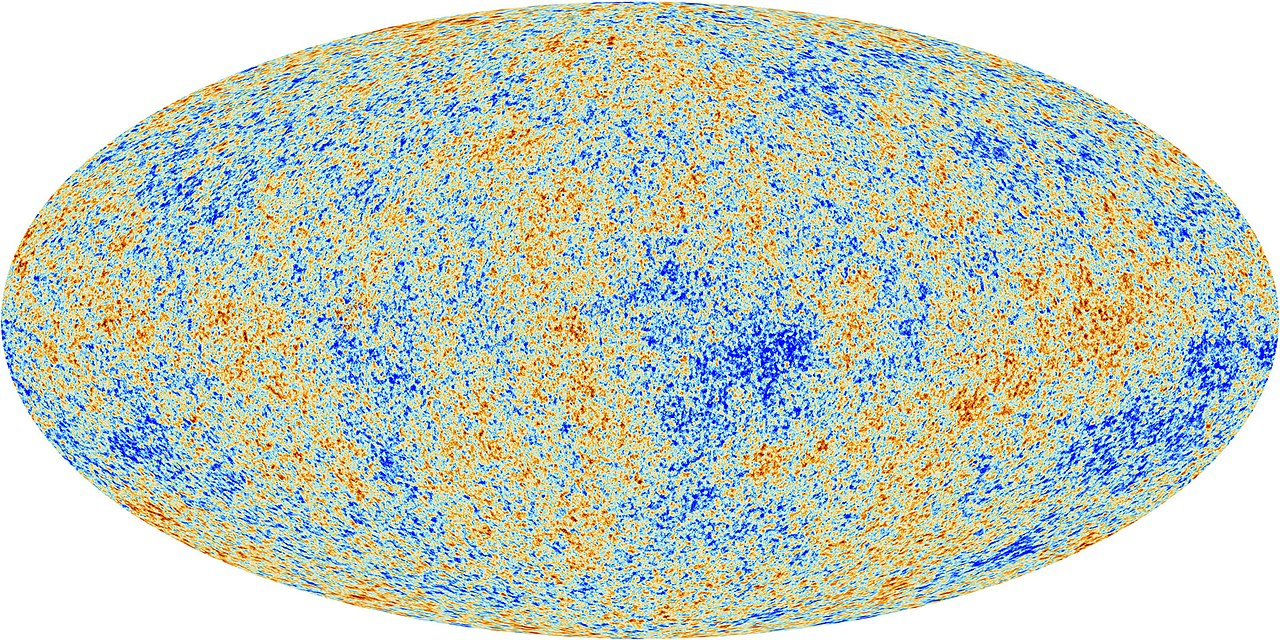
\includegraphics[width=0.9\linewidth]{Figuras/Artigo1/CMB.jpg}
	\caption{\small Mapa de calor da radiação cósmica de fundo (CMB). As regiões mais alaranjadas tem maior temperatura, enquanto as azuladas são mais frias. Fonte: \href{https://en.wikipedia.org/wiki/Cosmic_microwave_background}{Wikipédia}.}
	\label{fig:CMB}
\end{figure}

Mas o que diabos aconteceu com esses fótons vagantes, se nada mais havia para pará-los? A resposta é que eles andaram até onde conseguiram, e vários deles chegaram até a Terra. Sim, fótons/luz de 13,8 bilhões de anos chegaram até nós! Na verdade, a afirmação é mais forte ainda: luz de 13,8 bilhões de anos chegou até aqui na Terra, e está colidindo com você neste exato momento. Você está a todo momento sendo banhando de luz primordial!

Obviamente, quando fazemos afirmações fortes como ``luz primordial chegou até nós'', elas recebem um ar meio misterioso e até místico. Mas devo relembrá-lo de que este é um conceito científico: esta luz primordial já foi observada, e é essencial para a cosmologia moderna.

Chamamos essa luz, a mais antiga já vista pelo homem, de \textit{radiação cósmica de fundo} (CMB\footnote{Do inglês \textit{Cosmic Microwave Background Radiation}.}). Ela foi medida pela primeira vez por Penzias e Wilson em 1964 \ref{ref1:artigo1}.Na verdade, eles tentaram medir outro efeito, mas detectaram um sinal luminoso muito fraco, inicialmente atribuindo-o a falhas do equipamento. Na verdade, estavam descobrindo algo de muito profundo.

\begin{figure}[H]
	\centering
	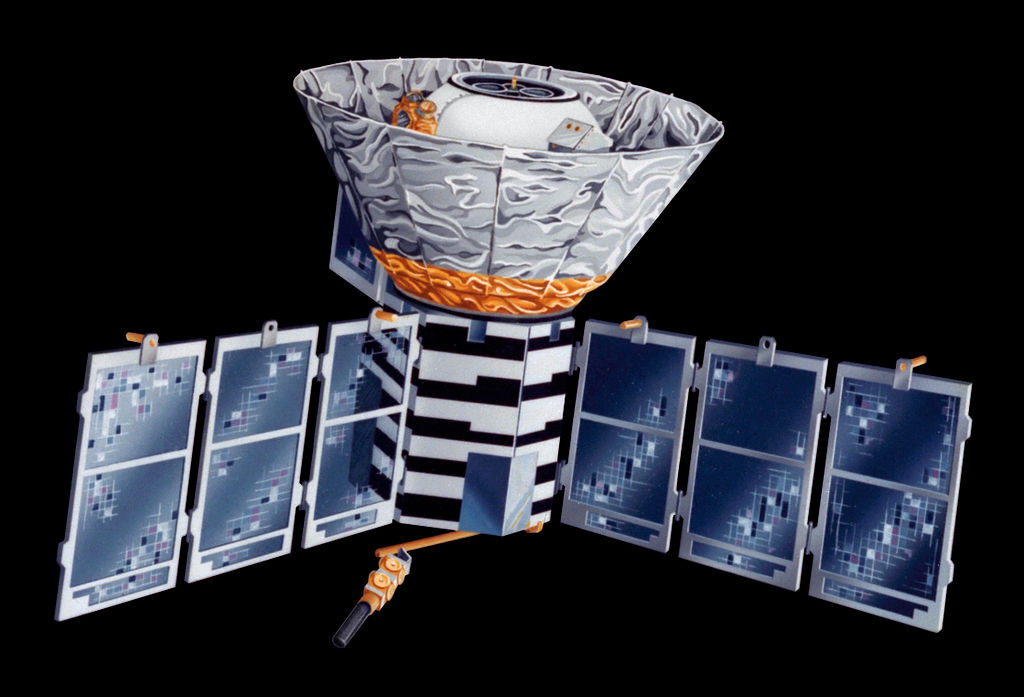
\includegraphics[width=0.8\linewidth]{Figuras/Artigo1/COBE.jpg}
	\caption{Satélite COBE, enviado para o espaço a fim de observar a CMB. Fonte: \href{https://en.wikipedia.org/wiki/List_of_cosmic_microwave_background_experiments\#/media/File:Cobe_vision1.jpg}{Wikipédia}.}
	\label{fig:COBE}
\end{figure}

Depois de sua primeira detecção, a CMB foi estudada por várias outras missões, pois ela é, no sentido mais literal da palavra, uma foto do universo primordial (ver Figura \ref{fig:CMB}). Através dela, podemos realmente fazer ``arqueologia'' com nosso universo e descobrir características que ele tinha há 13,8 bilhões de anos!

Atualmente, a CMB é tema de estudo de diversos pesquisadores no Brasil e no mundo. A quantidade de informação que ela nos dá sobre o universo primitivo é incrível, tanto que daria praticamente um outro texto aqui do Newston. Apenas para mencionar alguns satélites lançados para estudar a CMB, temos o COBE\footnote{\textit{Cosmic Microwave Background Explorer}. Ver Figura \ref{fig:COBE} .}(1989-1990), WMAP\footnote{\textit{Wilkinson Microwave Anisotropy Probe}.}(2001-2010), e Planck (2009-2013).



\mysubtitle{O Plasma Primordial}

Vimos então que, antes da Recombinação, não existiam sequer átomos no universo: os prótons e elétrons eram livres e, quando tentavam se juntar, eram separados por um fóton altamente energético.

Chamamos esse estado da matéria, no qual não há sequer átomos, de \textbf{plasma}. Porém, antes da Nucleossíntese Primordial, nem os núcleos dos átomos existiam. Mais precisamente, os prótons e nêutrons que os constituem estavam quebrados em seus componentes, os quarks e os glúons.

\begin{figure}[H]
	\centering
	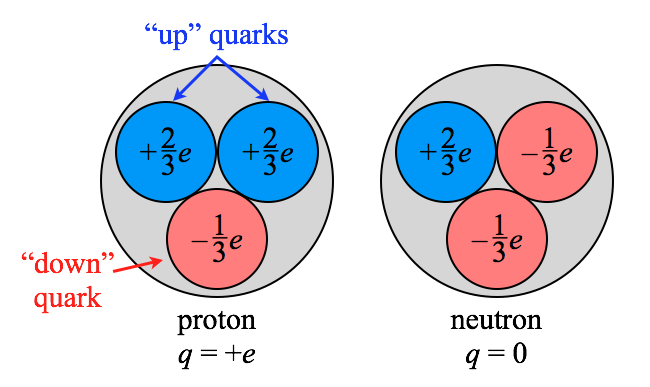
\includegraphics[width=\linewidth]{Figuras/Artigo1/quarks.png}
	\caption{Os prótons e nêutrons são feitos de quarks. Fonte: \href{https://5-volts.blogspot.com/2016/06/carga-eletrica.html}{An Introduction to Electricity and Magnetism}.}
	\label{fig:quarks}
\end{figure}

Chamamos então o estado do universo nessa época de um \textbf{plasma de quarks e glúons}. As outras partículas, como fótons, neutrinos e elétrons também estavam ali, mas o nome é dado porque quarks e glúons livres só ocorrem nesse estado da matéria.

Esse plasma pode então ser descrito como um grande carnaval, com partículas de todas as cores e sabores sambando em um frenezi louco nessa sopa primordial. Esse era o passado do Cosmos.

\mysubtitle{Mais problemas}

Quando observamos a CMB (Figura \ref{fig:CMB}), notamos uma coisa curiosa: ao longo de todo o céu, ela possui em média a mesma temperatura (cerca de 3 Kelvin, ou -270ºC). Isso é muito estranho pois, para que um sistema entre em equilíbrio térmico (atinja uma mesma temperatura), é necessário que diferentes partes dele tenham tido contato. Por exemplo, um cubo de gelo jamais derreterá se não for tirado da geladeira.


No caso da CMB, vemos então que regiões muito afastadas do céu têm a mesma temperatura. Mas elas não tiveram contato térmico: a luz de um lado não interagiu com a do outro lado para que todas tenham a mesma temperatura (ver Figura \ref{fig:horizon}). Esse fato não é bem compreendido pela cosmologia moderna, sendo conhecido como \textbf{Problema do Horizonte}.

Na verdade, há outros mistérios de nosso universo: assumimos que ele é espacialmente plano\footnote{Ele poderia ter curvatura espacial e ser uma 3-esfera, por exemplo}, mas por que haveria ele de ser assim?



Além disso, vemos um universo cheio de estruturas: galáxias, buracos negros, filamentos, planetas, sóis, aglomerados de galáxias, etc. Uma outra pergunta a ser respondida é: daonde vieram tais estruturas? Como elas se formaram?


\begin{figure}[H]
	\centering
	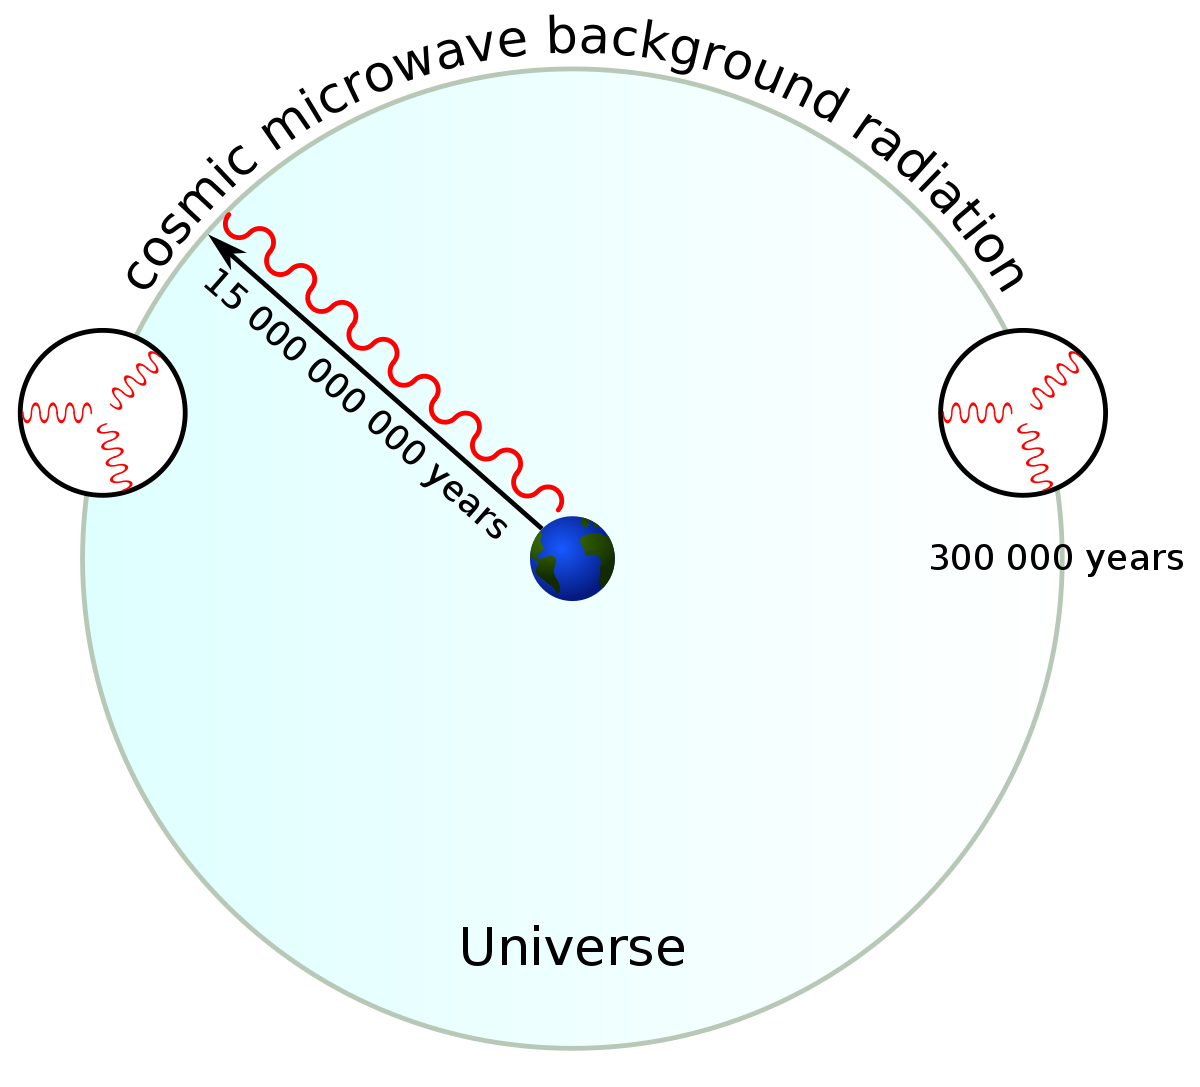
\includegraphics[width=\linewidth]{Figuras/Artigo1/horizon.png}
	\caption{Ao olharmos a CMB, vemos pontos de direções opostas(direita e esquerda) tem a mesma temperatura. Fonte: \href{https://www.pngwing.com/en/free-png-irtdi}{PNGwing}.}
	\label{fig:horizon}
\end{figure}

A resposta é que tais problemas... ainda não têm resposta. Mas há tentativas de resolvê-los. Uma das mais comuns é a chamada \textbf{Inflação}, que modifica a expansão do universo e resolve o problema do Horizonte e os outros em uma única tacada. Veremos isso no próximo texto da coleção: \textbf{Era Inflacionária}, aqui no Newston!

\authorinfo{Luiz Felipe Demétrio}{http://lattes.cnpq.br/3247376940028009}
% Use esse comando para adicionar o nome do autor(a) do artigo no final, e o link para o seu currículo lattes




\end{multicols}

